\documentclass[11pt]{article}
\usepackage[letterpaper, margin=1.1in]{geometry}
\usepackage{amssymb}
%\usepackage[ruled, vlined]{algorithm2e}
\usepackage{amsmath}
\usepackage{tikz}
\usetikzlibrary{calc}
\usepackage[font=footnotesize]{caption}
\usepackage{float}
\usepackage{mathtools}
\usepackage{mymath,gmech}

\newcommand{\TODO}[1]{\textcolor{red}{[TODO: #1]}}

\title{Ablation Study of Feature Replenishment Threshold $\tau_{fr}$}

\begin{document}

In the simulation, we conduct an ablation study about the influence of 
feature replenishment threshold $\tau_{fr}$. 
We use three trajectory tracking accuracy metrics: average lateral error (ALE),
terminal error (TE), and normalized path difference area (NPDA).
The details about these metrics refer to another supplemental material.
The number of feature trajectory regeneration per length is also recorded.
Outcomes of averages over all trajectory templates are included in 
Table \ref{tab:regThresh} and Fig. \ref{fig:regThresh}

With smaller $\tau_{fr}$, the performance of trajectory servoing becomes 
worse since it may servo with less number of tracked features. 
The control could be unstable and have oscillations. 
In contrast, if $\tau_{fr}$ is significantly large, trajectory servoing 
will more frequently trigger feature replenishment. 
Pose estimation errors could be involved to cause worse performance.
Therefore, a number in between is the best choice for $\tau_{fr}$. 
We used $\tau_{fr}=10$ in all of our experiments.

\TODO{add ale and double check if all values are up to date. Add ALE to the figure}

\begin{figure*}[h]
\begin{minipage}[t]{\textwidth}
\centering
%\vspace*{-1.45in}
\captionof{table}{ Raw data from ablation study of feature replenishment $\tau_{fr}$ \label{tab:regThresh}}
\vspace*{-0.5em}
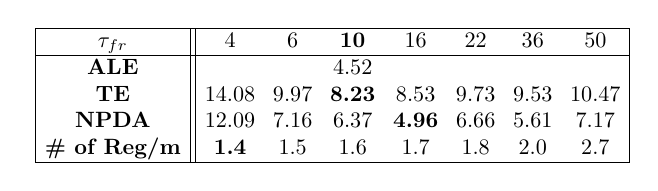
\begin{tikzpicture}[inner sep=0pt,outer sep=0pt,scale=1, every node/.style={scale=0.8}]
    % 
  \node[anchor=north west] (sim_thresh) at (0, 0pt)
  {
  \setlength{\tabcolsep}{4pt}
  \begin{tabular}{|c||ccccccc|}
  \hline 
  \textbf{$\tau_{fr}$} & 4 & 6 & \textbf{10} & 16 & 22 & 36 & 50 \\ 
  \hline 
  \textbf{ALE}  &  &  & 4.52 &  &  &  &  \\ 
  \textbf{TE}   & 14.08 & 9.97 & \textbf{8.23} & 8.53 & 9.73 & 9.53 & 10.47  \\ 
  \textbf{NPDA} & 12.09 & 7.16 & 6.37 & \textbf{4.96} & 6.66 & 5.61 & 7.17  \\ 
  \textbf{\# of Reg/m} & \textbf{1.4} & 1.5 & 1.6 & 1.7 & 1.8 & 2.0 & 2.7 \\ 
  \hline 
  \end{tabular}
  };       

\end{tikzpicture}
\end{minipage}
\vspace*{-0.5em}
\end{figure*}

\begin{figure*}[h]
\begin{minipage}[t]{0.49\textwidth}
\centering
\begin{tikzpicture}[inner sep=0pt,outer sep=0pt]
	  \node[anchor=south west] (pop) at (0in, 0in)
      {{\includegraphics[height=2.2in,clip=true,trim=0in 0in
      0in 0in]{figs/tau_num_reg.png}}};
\end{tikzpicture}
\end{minipage}
\hfill
\begin{minipage}[t]{0.49\textwidth}
\centering
\begin{tikzpicture}[inner sep=0pt,outer sep=0pt]
	  \node[anchor=south west] (pop) at (0in, 0in)
      {{\includegraphics[height=2.2in,clip=true,trim=0in 0in
      0in 0in]{figs/tau_npda_te.png}}};
\end{tikzpicture}
\end{minipage}
\vspace*{-0.5em}
\caption{Ablation study plots of feature replenishment $\tau_{fr}$ \label{fig:regThresh}}
\vspace*{-0.5em}
\end{figure*}

\end{document}